\documentclass[11pt a4paper]{article}
\usepackage[margin=2cm]{geometry}
\usepackage{amsmath, amssymb}
\usepackage{graphicx}
\usepackage{float}
\usepackage{aligned-overset}
\usepackage{subcaption}
\usepackage{tabularx} % fuer gleichungen nebeneinander
\usepackage{wrapfig} % damit figures neben text sien koennen

% partielle ableitungen
\newcommand{\delr}{\partial_r}
\newcommand{\delt}{\partial_t}
\newcommand{\deltheta}{\partial_\theta}
\newcommand{\delphi}{\partial_\varphi}

% elektrische feldkonstante
\newcommand{\epsz}{\epsilon_0}
% 1 / 4pi eps
\newcommand{\kco}{\frac{1}{4\pi\epsilon_0}}
% del fuer partial
\newcommand{\del}{\partial}

% div und rot
\newcommand{\diver}{\vec \nabla \cdot}
\newcommand{\rot}{\vec \nabla \times}

% hyperbolische funktionen
\newcommand{\arsinh}{\text{arsinh}}
\newcommand{\arcosh}{\text{arcosh}}
\newcommand{\artanh}{\text{artanh}}

% fuer impedanzen 
\newcommand{\omegaC}{\omega C}
\newcommand{\omegaL}{\omega L}
\newcommand{\omegaR}{\omega R}
\newcommand{\omegaLC}{\omega LC}
\newcommand{\omegaLCR}{\omega LCR}
\newcommand{\omegaCR}{\omega CR}

% fancy header
\usepackage{fancyhdr}
\fancyhf{}
% vspaces in den headern fuer Distanzen notwendig
% linke Seite: Namen der Abgabegruppe
\lhead{\textbf{Matthias Maile\\Roman Surma}\vspace{1.5cm}}
% rechte Seite: Modul, Gruppe, Semester
\rhead{\textbf{Physik II - Gruppe 2\\Sommersemester 2020}\vspace{1.5cm}}
% Center: nr. des blattes
\chead{\vspace{2.5cm}\huge{\textbf{21. Übungsblatt}}}
% benoetigt damit der eigentliche Text nicht in der Überschrift steckt
\setlength{\headheight}{4cm}

% zum zeichnen tikz
\usepackage{tikz}

% fuer fabigen text
\usepackage{xcolor}

% irgendwas mit figures
\usepackage{subcaption}

\begin{document}
\thispagestyle{fancy}

\section*{Aufgabe 1}
a) 
\begin{align*}
	Z_{AB}
	&= Z_C + Z_{LR} \\
	&= \frac{i\omega C} + \frac{i\omega LR}{i \omega L + R} \\
	&= \frac{i \omega L + R + i \omega C (i \omega LR)}{i \omegaC (i\omegaL + R)} \\
	&= \frac{R - \omega^2 LCR + i \omega L}{i\omega CR - \omega^2 LC}
\end{align*}
Für die relle Impedanz:
\begin{align*}
	\text{Im} \left( Z_{AB} \right)
	&= \frac{\omega L (- \omega^2 LC) - (R - \omega^2 LCR) \cdot \omegaCR}{(\omega CR)^2 + (\omega^2 LC)^2} 
	\overset{!}{=} 0 \\
	% bruch entfernen
	\Rightarrow
	0
	&= \omega L (- \omega^2 LC) - (R - \omega^2 LCR) \cdot \omegaCR \\
	% vereinfachen
	&= -\omega^3 L^2 C - \omega CR^2 + \omega^3 LC^2R^2 \\
	% durch omega teilen
	\Rightarrow
	0
	&= -\omega^2 L^2 C - CR^2 + \omega^2 LC^2R^2 \\
	\Leftrightarrow
	CR^2
	&= -\omega^2 L^2 C + \omega^2 LC^2R^2 \\
	% nach omega^2 umstellen
	\Rightarrow
	\omega^2
	&= \frac{CR^2}{L^2C^2R^2 - L^2C} \\
	\Rightarrow
	\omega
	&= \sqrt{\frac{R^2}{L^2CR^2 - L^2}}
\end{align*}
b) Die an der LCR-Schaltung abfallende Spannung $U_{AB}$ ist bestimmt durch
\[ U_{AB} = \frac{Z_{AB}}{R_i + Z_{AB}} U_0 \]
Dann lautet die elektrische Leistung der LCR-Schaltung:
\begin{align*}
	P
	&= \frac{\Delta U^2}{Z_{AB}} \\
	&= \frac{Z_{AB}^2}{(R_i+Z_{AB})^2} \frac{1}{Z_{AB}} U_0 \\
	&= \frac{Z_{AB}}{(R_i+Z_{AB})^2} U_0 
\end{align*}
Diese wird maximal für
\begin{align*}
	d_{Z_{AB}} P
	&= U \frac{(R_i+Z_{AB})^2 - Z_{AB} \cdot 2 \cdot (R_i + Z_{AB})}{(R_i+Z_{AB})^4} \overset != 0 \\
	\Leftrightarrow
	0
	&= R_i + Z_{AB} - 2 Z_{AB} \\
	\Rightarrow
	Z_{AB} &= R_i
\end{align*}

\newpage
\setlength{\headheight}{0cm}

c) 
\begin{align*}
	R_i
	&= \frac{R - \omega^2 LCR + i \omega L}{i\omega CR - \omega^2 LC} \\
	% quotient berechnen
	Z_{AB} \in \mathbb{R} \Rightarrow
	&= \frac{(R - \omega^2 LCR) (-\omega^2 LC) + \omega^2 LCR}{(\omega CR)^2 + (\omega^2 LC)^2} \\
	&= \frac{\omega^4 L^2 C^2 R - \omega^2 LCR + \omega^2 LCR}{(\omega CR)^2 + (\omega^2 LC)^2} \\
	&= \frac{\omega^4 L^2 C^2 R}{(\omega CR)^2 + (\omega^2 LC)^2} \\
	&= \frac{\omega^2 L^2 R}{R^2 + \omega^2 L^2} \\
	% nach 0 umstellen
	\Rightarrow
	0
	&= \frac{\omega^2 L^2 R}{R^2 + \omega^2 L^2} - R_i \\
	% bruch entfernen
	\Leftrightarrow
	0
	&= \omega^2 L^2 R - R_iR^2 - R_i\omega^2L^2 \\
	% fuer pq formel
	\Leftrightarrow
	0
	&= R^2 - \frac{\omega^2L^2}{R_i} R + \omega^2 L^2
\end{align*}
Mit der pq-Formel erhalten wir eine Lösung:
\[
	R = \frac{\omega^2L^2}{2 R_i} \pm \sqrt{\left( \frac{\omega^2L^2}{2 R_i}\right)^2 - \omega^2 L^2} 
\]


\newpage
\setlength{\headheight}{0cm}

\section*{Aufgabe 2}
a) Der Aufbau sieht entsprechend aus:
\begin{figure}[H]
	\centering
	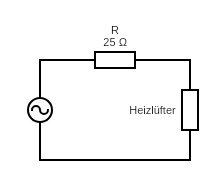
\includegraphics[width = 5cm]{figures/aufgabe2-1.png}
\end{figure}
\noindent
Für die Betriebsleistung muss ein Strom $I$ fließen:
\[ P_H = U_H \cdot I \ \Rightarrow \ I = \frac{P_H}{U_H} \approx 7.8261 \ A \]
Da dieser Strom auch durch den Widerstand fließt, wird an diesem die Arbeit geleistet:
\[ P_R = U_R \cdot I = R \cdot I^2 = 1531.2 \ W \]
Gesamtleistung und Wirkungsgrad lauten somit
\[ 
	P_G = P_H + P_R = 3331.2 \ W
	\Rightarrow
	\eta = \frac{P_H}{P_G} \approx 0.54
\]
b) Mit den Transformatoren sieht der Aufbau wie folgt aus:
\begin{figure}[H]
	\centering
	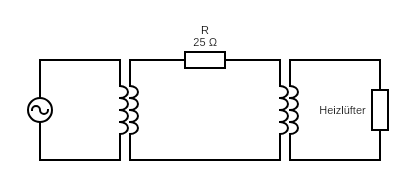
\includegraphics[width = 8cm]{figures/aufgabe2-2.png}
\end{figure}
\noindent
Aus dem Windungszahlverhältnis $9:1$ folgt das Stromverhältnis 
\[ I_R : I_H = 1 : 9 \ \Rightarrow I_R = \frac{I_H}{9} \approx 0.87 \ A \]
Damit muss am Widerstand die Leistung $P_R^\prime$ geleistet werden:
\[ P_R^\prime = R \cdot I_R^2 = 18.904 \ W \]
Gesamtleistung und Wirkungsgrad lauten somit
\[ 
	P_G^\prime = P_H + P_H^\prime = 1818.9 \ W
	\ \Rightarrow \
	\eta^\prime = \frac{P_H}{P_G^\prime} \approx 0.99
\]

\newpage

\section*{Aufgabe 3}
a) Da die Leitung einen Widerstand besitzt, verrichtet der Strom an diesem Arbeit durch Aufheizen des Kabels.
\[ P = U \cdot I = I^2 \cdot R \]
Dieser ist proportional zum Quadrat der Stromstärke $I$, d.h. diese sollte minimiert werden. Dafür muss die 
Spannung $U$ angehoben werden.
\newline
b)
\[
	P = I^2 \cdot R = 500^2 \ A^2 \cdot 0.2 \ k\Omega = 5 \cdot 10^4 \ W
\]

\section*{Aufgabe 4}
a) Mit der 4. Maxwellgleichung wissen wir, dass 
\[ \oint_{\del A} \vec B \cdot d\vec s = \mu_0 (I + I_V) \]
und diese Gleichung auch für alle Flächen erfüllt sein muss. \\
Wenn wir als uns eine Fläche denken, wo der Leiter komplett durch die Fläche durchstößt, also kein 
Verschiebungsstrom existiert, so muss gelten:
\[ \oint_{\del A} \vec B \cdot d\vec s = \mu_0 I. \]
Genauso kann man aber auch eine Fläche wählen, die, am Leiter vorbei, durch den Raum des Kondensators verläuft.
Durch diese Fläche fließt dann kein Strom, sondern nur ein Verschibungsstrom. Da wir aber den Rand gleich ließen, 
können wir für $I_V$ schreiben:
\[ \oint_{\del A} \vec B \cdot d \vec s = \mu_0 I = \mu_0 I_V \ \Rightarrow \ I_V = I = 2 \ A \]
b) Das elektrische Feld des Plattenkondensators ist gegeben durch
\[ E(t) = \frac{\sigma(t)}{\epsz} \] 
mit $\sigma$ als Flächenladungsdichte $\frac{Q}{A}$. \\
Dann lautet die Ableitung des $\vec E$-Feldes nach der Zeit:
\begin{align*}
	\delt E(t) 
	&= \delt \frac{\sigma}{\epsz} \\
	% sigma einsetzen
	&= \delt \frac{Q}{A \cdot \epsz} \\
	&= \frac{I}{A \cdot \epsz} \\
	&= \frac{2 \ A}{\epsz}
\end{align*}
c) Der Verschiebungsstrom $\tilde{I}_V$, der durch die Fläche $A^\prime$ fließt, lässt sich dann bestimmen:
\begin{align*}
	\tilde{I}_V
	&= \epsz \delt \int_{A^\prime} \vec E \cdot d \vec A^\prime \quad 
	\vec E \text{ homogen} \\
	&= \epsz \delt E \cdot A^\prime \\
	&= \epsz A^\prime \frac{I}{\epsz A} \\
	&= \frac{A^\prime}{A} I \\
	&= \frac{I}{4}
\end{align*}
d) Aus der 4. Maxwell-Gleichung folgt dann das Megnetfeld am Rand der der Fläche $A^\prime$:
\[ \oint_{A^\prime} \vec B \cdot d\vec s = \mu_0 (I + I_V) = \mu_0 I_V = \mu_0 \frac{I}{4} \]

\newpage

\section*{Aufgabe 5}
a) 
\begin{enumerate}
	\item Mit Gaußschem Satz
	\[ 
		\diver \vec E = \frac{\rho}{\epsz} 
		\Rightarrow
		\int_V \diver \vec E \ dV = \int_V \frac{\rho}{\epsz} \ dV 
		\Rightarrow
		\oint_{\partial_V} \vec E \ d\vec A = \int_V \frac{\rho}{\epsz} \ dV 
		= \frac{q_\text{enq}}{\epsz}
	\]
	\item Ebenfalls mit Gaußschem Satz
	\[
		\diver \vec B = 0
		\Rightarrow
		\int_V \diver \vec B \ dV = 0
		\Rightarrow
		\oint_{\partial_V} \vec B \ d\vec A = 0
	\]
	\item Mit Satz von Stokes
	\[
		\rot \vec E = -\delt \vec B
		\Rightarrow
		\int_A \rot \vec E \ d\vec A = \int_A -\delt \vec B \ d\vec A
		\Rightarrow
		\oint_{\partial_A} \vec E \ d\vec r = -\delt \int_A \vec B \ \vec d\vec A = -\delt \phi
	\]
	\item Mit Satz von Stokes
	\[ 
	\rot \vec B = \mu_0 \vec j + \mu_0 \epsz \delt \vec E 
	\Rightarrow
	\int_A \rot \vec B \cdot d\vec A
	= \oint_{\del A} \vec B \cdot d\vec r
	= \mu_0 \int_A \vec j \cdot d\vec A + \mu_0 \epsz \int_A \delt \vec E \cdot d\vec A
	= \mu_0 I_\text{enq} + \mu_0 \epsz \int_A \delt \vec E \cdot d\vec A
	\]
\end{enumerate}
b) Aus der 4. Maxwell-Gleichung erhalten wir:
\begin{align*}
	\rot \vec B 
	&= \mu_0 \vec j + \mu_0 \epsz \delt \vec E \\
	% auf beiden Seiten divergenz
	\Rightarrow
	\underbrace{\diver \left(\rot \vec B \right)}_{=0}
	&= \mu_0 \diver \vec j + \mu_0 \epsz \diver \left( \delt \vec E \right) \\
	% umstellen nach div \dot E
	\Rightarrow
	\diver \dot{\vec E}
	&= - \frac{\diver \vec j}{\epsz} \tag{5.1}
\end{align*}
Ausgehend von (5.1) und der Kontinuitätsgleichung lässt sich dann zeigen:
\begin{align*}
	\diver \vec E(t) 
	&= \diver \vec E(0) + \int_0^t \diver \dot{\vec E} \ dt \\
	% umformen mit 5.1
	(5.1) \Rightarrow \quad
	&= \frac{\rho(0)}{\epsz} - \int_0^t \frac{\diver \vec j}{\epsz} \ dt \\
	   % koninuitaet
	\text{(Kontinuität)} \Rightarrow \quad
	&= \frac{\rho(0)}{\epsz} + \int_0^t \frac{\delt \rho}{\epsz} \ dt \\
	&= \frac{\rho(0)}{\epsz} + \left. \frac{\rho(t)}{\epsz} \right|_0^t \\
	&= \frac{\rho(0)}{\epsz} + \left. \frac{\rho(t)}{\epsz} \right|_0^t \\
	&= \frac{\rho(0)}{\epsz} + \frac{\rho(t)}{\epsz} - \frac{\rho(0)}{\epsz} \\
	&= \frac{\rho(t)}{\epsz}
\end{align*}
Mit der 2. und 3. Maxwellgleichug lässt sich zeigen:
\begin{align*}
	\diver \vec B(t) 
	&= \diver \vec B(0) + \int_0^t \diver \dot{\vec B}(t) \ dt \\
	&= \diver \vec B(0) - \int_0^t \diver \left( \rot E(t) \right) \ dt \\
	&= \diver \vec B(0) \\
	&= 0
\end{align*}

\end{document}
